\section{MARCO TEÓRICO}

Esta sección fundamenta los conceptos matemáticos, estadísticos y computacionales que sustentan las decisiones metodológicas adoptadas en el proyecto, detallando la semántica de los datos y la formulación analítica de los algoritmos de aprendizaje no supervisado.

\subsection{Diccionario de Datos: Inteligencia Urbana y Criminalidad}

El proyecto integra dos fuentes complementarias: el dataset masivo de referencia del Departamento de Policía de Chicago (\textit{Chicago Police Department} -- CPD) y el corpus georreferenciado de crónicas de prensa de seguridad ciudadana de Bolivia.

\subsubsection{Diccionario Original (Fuentes en Bruto)}

El dataset primario de Chicago (\texttt{Crimes\_-\_2020\_to\_Present.csv}) comprende más de $800.000$ observaciones en bruto con 30 atributos registrados desde el año 2020:
\begin{itemize}
    \item \textbf{ID / Case Number:} Identificador numérico único de la base de datos CPD y código alfanumérico del reporte del caso.
    \item \textbf{Date:} Marca temporal completa del incidente (formato MM/DD/YYYY hh:mm:ss AM/PM).
    \item \textbf{Block:} Dirección aproximada a nivel de centena de bloque (anonimización por protección de datos).
    \item \textbf{IUCR (\textit{Illinois Uniform Crime Reporting}):} Código normalizado de cuatro dígitos que clasifica con precisión la infracción legal según la legislación del estado de Illinois.
    \item \textbf{Primary Type:} Categoría general del delito (ej. \textit{THEFT}, \textit{BATTERY}, \textit{ROBBERY}, \textit{ASSAULT}, \textit{NARCOTICS}).
    \item \textbf{Description:} Subclasificación detallada del hecho (ej. \textit{\$500 AND UNDER}, \textit{SIMPLE}, \textit{ARMED: HANDGUN}).
    \item \textbf{Location Description:} Entorno físico o tipología del predio donde acaeció el delito (ej. \textit{STREET}, \textit{RESIDENCE}, \textit{SIDEWALK}, \textit{COMMERCIAL / BUSINESS}).
    \item \textbf{Arrest:} Booleano que indica si la intervención culminó en la detención del sospechoso (\textit{True / False}).
    \item \textbf{Domestic:} Booleano que indica si el delito califica como violencia intrafamiliar según el acta (\textit{True / False}).
    \item \textbf{Beat:} Cuadrante de patrullaje táctico territorial más pequeño de la policía.
    \item \textbf{District:} Distrito policial numerado (Chicago cuenta con 22 distritos policiales activos).
    \item \textbf{Ward / Community Area:} Divisiones políticas (distrito electoral) y comunidades barriales socioeconómicas (77 áreas comunitarias de Chicago).
    \item \textbf{X Coordinate / Y Coordinate:} Coordenadas planas en pies proyectadas según el sistema \textit{State Plane Illinois East (NAD83)}.
    \item \textbf{Latitude / Longitude:} Coordenadas geodésicas en grados decimales (elipsoide WGS84).
\end{itemize}

El corpus de Bolivia (\texttt{data\_noticias\_bolivia.csv}), construido mediante extracción automatizada sobre la prensa digital nacional (rotativos del eje troncal y periódicos departamentales de los 9 departamentos), registra:
\begin{itemize}
    \item \textbf{id:} Identificador secuencial del reporte periodístico.
    \item \textbf{fecha:} Fecha de publicación de la noticia (formato AAAA-MM-DD).
    \item \textbf{titular:} Encabezado periodístico del hecho delictivo.
    \item \textbf{medio:} Diario o agencia emisora (ej. \textit{El Deber}, \textit{Los Tiempos}, \textit{La Razón}, \textit{Correo del Sur}, \textit{El Potosí}, \textit{La Patria}, \textit{El País}).
    \item \textbf{departamento:} Jurisdicción departamental en Bolivia (La Paz, Santa Cruz, Cochabamba, Oruro, Potosí, Chuquisaca, Tarija, Beni, Pando).
    \item \textbf{ciudad:} Municipio o localidad específica del suceso.
    \item \textbf{categoria:} Clasificación periodística inicial del suceso (ej. \textit{Seguridad}, \textit{Policial}, \textit{Sucesos}).
    \item \textbf{latitud / longitud:} Coordenadas geodésicas asignadas mediante gazetteers urbanos georreferenciados.
    \item \textbf{texto:} Crónica periodística completa con detalles del \textit{modus operandi}, armamento y desenlace.
\end{itemize}

\subsubsection{Diccionario de Datos Después de la Limpieza y Preprocesamiento}

Tras la ejecución del pipeline de preparación, optimización de tipos y extracción de características, los datasets estructurados para el modelado no supervisado presentan el esquema consolidado de la Tabla \ref{tab:diccionario_limpio}:

\begin{table}[htbp]
\centering
\small
\begin{tabularx}{\textwidth}{l p{3.5cm} l X}
\toprule
\textbf{Variable} & \textbf{Tipo de Dato} & \textbf{Dominio} & \textbf{Definición y Rol en el Modelo} \\
\midrule
\texttt{lat} & Float64 & $[-90.0, 90.0]$ & Latitud geodésica limpia. \\
\texttt{lon} & Float64 & $[-180.0, 180.0]$ & Longitud geodésica limpia. \\
\texttt{lat\_rad} & Float64 & Radianes & Latitud en radianes para cálculo directo de \textit{Haversine}. \\
\texttt{lon\_rad} & Float64 & Radianes & Longitud en radianes para cálculo directo de \textit{Haversine}. \\
\texttt{hour\_sin} & Float32 & $[-1.0, 1.0]$ & Componente senoidal del ciclo horario: $\sin(2\pi \cdot \text{hora}/24)$. \\
\texttt{hour\_cos} & Float32 & $[-1.0, 1.0]$ & Componente cosenoidal del ciclo horario: $\cos(2\pi \cdot \text{hora}/24)$. \\
\texttt{dow\_sin} & Float32 & $[-1.0, 1.0]$ & Componente senoidal del día de la semana: $\sin(2\pi \cdot \text{dow}/7)$. \\
\texttt{dow\_cos} & Float32 & $[-1.0, 1.0]$ & Componente cosenoidal del día de la semana: $\cos(2\pi \cdot \text{dow}/7)$. \\
\texttt{is\_weekend} & Int8 & $\{0, 1\}$ & Indicador binario de fin de semana (Sábado/Domingo = 1). \\
\texttt{arrest} & Int8 & $\{0, 1\}$ & Estatus binario de arresto ($1 = \text{Arresto efectivo}$). \\
\texttt{domestic} & Int8 & $\{0, 1\}$ & Estatus binario de violencia intrafamiliar ($1 = \text{Doméstico}$). \\
\texttt{primary\_type} & Category & 33 clases & Tipología criminal principal unificada. \\
\texttt{text\_clean} & String & Texto libre & Fusión normalizada de descripción y locación para NLP. \\
\texttt{district\_id} & Category & 22 distritos & Identificador del distrito policial para clustering jerárquico. \\
\bottomrule
\end{tabularx}
\caption{Diccionario de variables estructuradas listas para modelado no supervisado.}
\label{tab:diccionario_limpio}
\tablenote{Elaboración propia a partir de la ingeniería de variables sobre el benchmark CPD de Chicago y el corpus geocodificado de prensa de Bolivia. Las variables cíclicas se normalizan en el rango $[-1, 1]$ mediante componentes ortogonales y las coordenadas geográficas se expresan en radianes para cómputo geodésico directo.}
\end{table}

\subsubsection{Mapeo Departamental y Ecosistema de Medios Informativos de Bolivia}

La extracción y minería de texto sobre la seguridad ciudadana en Bolivia requirió estructurar un inventario exhaustivo de fuentes de información abiertas (OSINT). Dado que el país no cuenta con una base de datos abierta centralizada de denuncias policiales, se sistematizaron los rotativos y cadenas de mayor penetración editorial en el eje troncal y los seis departamentos restantes, tal como sintetiza la Tabla \ref{tab:medios_bolivia}:

\begin{table}[htbp]
\centering
\small
\begin{tabularx}{\textwidth}{l p{3.2cm} l X}
\toprule
\textbf{Jurisdicción} & \textbf{Medio Informativo} & \textbf{Portal Web Oficial} & \textbf{Canal YouTube / Identificador} \\
\midrule
Nacional (TV) & Bolivia TV (BTv) & \texttt{boliviatv.bo} & \texttt{@BoliviaTvMul} \\
Nacional (TV) & Unitel Bolivia & \texttt{unitel.bo} & \texttt{@unitel-bolivia} \\
Nacional (TV) & Red Uno de Bolivia & \texttt{reduno.com.bo} & \texttt{@redunotv} \\
Nacional (TV) & Red ATB & \texttt{atb.com.bo} & \texttt{@ATBEnConexion} \\
Nacional (Radio) & Erbol Digital & \texttt{erbol.com.bo} & \texttt{@rederbol} \\
Nacional (Radio) & Radio Panamericana & \texttt{panamericana.bo} & \texttt{@radio.panamericana} \\
Nacional (Agencia) & Agencia Fides (ANF) & \texttt{noticiasfides.com} & \texttt{@agenciadenoticiasfides2497} \\
La Paz & La Razón / El Diario & \texttt{larazon.bo} & \texttt{@LaRazónDigitalBolivia} \\
Santa Cruz & El Deber / El Día & \texttt{eldeber.com.bo} & \texttt{@webeldeber1} \\
Cochabamba & Los Tiempos / Opinión & \texttt{lostiempos.com} & \texttt{@lostiemposbol} \\
Chuquisaca & Correo del Sur & \texttt{correodelsur.com} & \texttt{@correodelsuryt} \\
Oruro & La Patria & \texttt{lapatria.bo} & \texttt{@PeriódicoLaPatriaBolivia} \\
Potosí & El Potosí / Kollasuyo & \texttt{elpotosi.net} & \texttt{@el.potosi} \\
Tarija & El País / La Voz & \texttt{elpais.bo} & \texttt{@elpaisbo} \\
Beni & La Palabra del Beni & \texttt{lapalabradelbeni.com} & \texttt{@benitvenlinea} \\
Pando & Sol de Pando & \texttt{soldepando.com} & \texttt{Sol de Pando Oficial} \\
\bottomrule
\end{tabularx}
\caption{Ecosistema de medios y fuentes periodísticas georreferenciadas de Bolivia.}
\label{tab:medios_bolivia}
\tablenote{Elaboración propia a partir del levantamiento documental consolidado en \texttt{NOTICIAS.md}. Comprende agencias estatales, redes privadas, emisoras de radio e impresos departamentales de los 9 departamentos del Estado Plurinacional de Bolivia.}
\end{table}

\subsection{Algoritmos No Supervisados Aplicados}

\subsubsection{K-Means Particional y Variantes Semánticas}

El algoritmo K-Means particiona un conjunto de $N$ observaciones $X = \{x_1, \dots, x_N\} \subset \mathbb{R}^D$ en $k$ clústeres disjuntos $S = \{S_1, \dots, S_k\}$ minimizando la inercia intra-clúster (\textit{Within-Cluster Sum of Squares} -- WSS):
\begin{equation}
    J(S) = \sum_{j=1}^k \sum_{x \in S_j} \| x - \mu_j \|^2
\end{equation}
donde $\mu_j = \frac{1}{|S_j|} \sum_{x \in S_j} x$ es el baricentro geométrico del clúster $S_j$. Para evitar mínimos locales subóptimos, se emplea la inicialización probabilística K-Means++ \cite{arthur2007}, cuya probabilidad de seleccionar un centro inicial $x$ es proporcional a $D(x)^2$, siendo $D(x)$ la distancia al centroide más próximo ya elegido.

\subsubsection{DBSCAN con Métrica Geodésica de Haversine}

DBSCAN (\textit{Density-Based Spatial Clustering of Applications with Noise}) \cite{ester1996} descubre agrupaciones espaciales basadas en la conectividad por densidad. Dado un radio de vecindad $\varepsilon$ y un umbral mínimo de puntos $MinPts$:
\begin{itemize}
    \item Un punto $p$ es \textbf{punto núcleo} (\textit{Core Point}) si su vecindad cerrada $N_\varepsilon(p) = \{q \in X \mid d(p,q) \le \varepsilon\}$ cumple $|N_\varepsilon(p)| \ge MinPts$.
    \item Un punto $q$ es \textbf{directamente alcanzable por densidad} desde $p$ si $q \in N_\varepsilon(p)$ y $p$ es punto núcleo.
    \item Los puntos que no son alcanzables por densidad desde ningún núcleo son clasificados formalmente como \textbf{ruido (etiqueta $-1$)}.
\end{itemize}

En lugar de distancias euclidianas planas que falsean distancias en la esfera terrestre, se aplica la \textbf{fórmula de Haversine} sobre coordenadas geográficas expresadas en radianes $(\phi_1, \lambda_1)$ y $(\phi_2, \lambda_2)$:
\begin{equation}
    d(p_1, p_2) = 2 R \arcsin \left( \sqrt{\sin^2\left(\frac{\Delta\phi}{2}\right) + \cos\phi_1 \cos\phi_2 \sin^2\left(\frac{\Delta\lambda}{2}\right)} \right)
\end{equation}
donde $R = 6371.0088 \text{ km}$ representa el radio medio volumétrico de la Tierra. El parámetro $\varepsilon$ se expresa en radianes mediante $\varepsilon_{\text{rad}} = \frac{d_{\text{km}}}{R}$.

\subsubsection{HDBSCAN: Clustering Jerárquico por Densidad y Persistencia}

HDBSCAN (\textit{Hierarchical DBSCAN}) \cite{campello2013} supera la principal limitación de DBSCAN (la incapacidad de manejar densidades dispares simultáneas en una misma ciudad). HDBSCAN define la \textbf{distancia de alcanzabilidad mutua} (\textit{Mutual Reachability Distance}):
\begin{equation}
    d_{\text{mreach-}k}(a, b) = \max \left\{ d_{\text{core-}k}(a), \, d_{\text{core-}k}(b), \, d(a, b) \right\}
\end{equation}
donde $d_{\text{core-}k}(a)$ es la distancia al $k$-ésimo vecino más próximo de $a$. Construye el Árbol de Expansión Mínima (\textit{Minimum Spanning Tree} -- MST) ponderado por esta métrica, genera una jerarquía continua y condensa el dendrograma bajo un umbral de tamaño mínimo de clúster ($min\_cluster\_size$). La extracción de los clústeres óptimos maximiza la persistencia o estabilidad del exceso de masa:
\begin{equation}
    S(C_i) = \sum_{p \in C_i} (\lambda_p - \lambda_{\text{birth}}(C_i))
\end{equation}
con $\lambda = \frac{1}{\varepsilon}$, seleccionando aquellos clústeres que perduran a lo largo de un espectro más amplio de densidades.

\subsubsection{OPTICS: Diagrama de Alcanzabilidad y Detección de Valles}

OPTICS (\textit{Ordering Points To Identify the Clustering Structure}) \cite{ankerst1999} extiende el concepto de densidad sin requerir un $\varepsilon$ rígido. Registra dos distancias fundamentales para cada punto:
\begin{equation}
    d_{\text{core}}(p) = \begin{cases} \text{INDEFINIDO} & \text{si } |N_\varepsilon(p)| < MinPts \\ \text{distancia al } MinPts\text{-ésimo vecino} & \text{en caso contrario} \end{cases}
\end{equation}
\begin{equation}
    d_{\text{reach}}(q, p) = \begin{cases} \text{INDEFINIDO} & \text{si } |N_\varepsilon(p)| < MinPts \\ \max \{ d_{\text{core}}(p), \, d(p, q) \} & \text{en caso contrario} \end{cases}
\end{equation}
El algoritmo produce un orden lineal de los datos que genera el \textbf{Gráfico de Alcanzabilidad} (\textit{Reachability Plot}), en el cual las depresiones o valles corresponden a clústeres compactos y las cúspides representan separaciones o regiones de baja densidad. Mediante el parámetro $\xi$ de inclinación, se extraen automáticamente clústeres anidados.

\subsubsection{Gaussian Mixture Models (GMM) y Esperanza-Maximización (EM)}

Los Modelos de Mixturas de Gaussianas formulan una densidad de probabilidad continua multivariante como una combinación convexa de $K$ distribuciones normales:
\begin{equation}
    p(x) = \sum_{k=1}^K \pi_k \, \mathcal{N}(x \mid \mu_k, \Sigma_k), \quad \text{con } \sum_{k=1}^K \pi_k = 1, \; \pi_k \ge 0
\end{equation}
donde $\mathcal{N}(x \mid \mu_k, \Sigma_k) = \frac{1}{(2\pi)^{D/2} |\Sigma_k|^{1/2}} \exp\left(-\frac{1}{2} (x-\mu_k)^T \Sigma_k^{-1} (x-\mu_k)\right)$. Los parámetros $\{\pi_k, \mu_k, \Sigma_k\}$ se optimizan mediante el algoritmo Esperanza-Maximización (EM):
\begin{itemize}
    \item \textbf{Paso E (Expectation):} Calcula la probabilidad posterior o responsabilidad de que el componente $k$ haya generado la observación $x_i$:
    \begin{equation}
        \gamma_{ik} = \frac{\pi_k \mathcal{N}(x_i \mid \mu_k, \Sigma_k)}{\sum_{j=1}^K \pi_j \mathcal{N}(x_i \mid \mu_j, \Sigma_j)}
    \end{equation}
    \item \textbf{Paso M (Maximization):} Actualiza los parámetros ponderados por las responsabilidades:
    \begin{equation}
        \mu_k^{\text{nuevo}} = \frac{\sum_{i=1}^N \gamma_{ik} x_i}{\sum_{i=1}^N \gamma_{ik}}, \quad \Sigma_k^{\text{nuevo}} = \frac{\sum_{i=1}^N \gamma_{ik} (x_i - \mu_k)(x_i - \mu_k)^T}{\sum_{i=1}^N \gamma_{ik}}, \quad \pi_k^{\text{nuevo}} = \frac{1}{N} \sum_{i=1}^N \gamma_{ik}
    \end{equation}
\end{itemize}
La descomposición espectral de la matriz de covarianza $\Sigma_k = V \Lambda V^T$ determina la orientación y magnitudes de los semiejes de las elipses de riesgo a $2\sigma$, abarcando teóricamente el $95.4\%$ de la masa de incidentes del clúster.

\subsubsection{Clustering Jerárquico Aglomerativo (Ward)}

El agrupamiento jerárquico aglomerativo sigue una estrategia ascendente (\textit{bottom-up}) que comienza con cada instancia como un clúster individual y fusiona sucesivamente el par de grupos más cercano. El criterio de **Ward** minimiza el incremento en la suma total de cuadrados de las distancias respecto al centroide fusionado:
\begin{equation}
    \Delta ESS(A, B) = \frac{|A| \cdot |B|}{|A| + |B|} \| \mu_A - \mu_B \|^2
\end{equation}
Este método preserva grupos balanceados y de mínima varianza interna, resultando ideal para la tipificación comparada de zonas urbanas y distritos policiales.

\subsubsection{Reducción de Dimensionalidad (PCA, SVD, PPCA, t-SNE, UMAP)}

Para proyectar y visualizar matrices dispersas de texto y espacios multivariables continuos, se articulan cinco técnicas:
\begin{itemize}
    \item \textbf{PCA (Principal Component Analysis):} Proyección lineal ortogonal que maximiza la varianza proyectada a través de los autovectores de la matriz de covarianza $\Sigma_X v_i = \lambda_i v_i$.
    \item \textbf{TruncatedSVD (LSA):} Descomposición en valores singulares sobre matrices dispersas TF-IDF $X \approx U_k \Sigma_k V_k^T$ sin requerir el centrado denso de la matriz, evitando saturación de memoria.
    \item \textbf{PPCA (Probabilistic PCA vía Factor Analysis):} Modelo de variables latentes gaussianas $x = W z + \mu + \epsilon$, con $z \sim \mathcal{N}(0, I)$ y ruido $\epsilon \sim \mathcal{N}(0, \Psi)$.
    \item \textbf{t-SNE \cite{vandermaaten2008}:} Mapeo probabilístico no lineal que preserva vecindades locales minimizando la divergencia de Kullback-Leibler $KL(P \parallel Q)$ entre similitudes gaussianas en alta dimensión y probabilidades según una distribución t-Student en baja dimensión:
    \begin{equation}
        q_{ij} = \frac{(1 + \|y_i - y_j\|^2)^{-1}}{\sum_k \sum_{l \neq k} (1 + \|y_k - y_l\|^2)^{-1}}
    \end{equation}
    \item \textbf{UMAP \cite{mcinnes2018}:} Técnica no lineal fundamentada en topología algebraica y geometría riemanniana que preserva tanto las distancias locales como las globales con una velocidad de cálculo sustancialmente superior a t-SNE.
\end{itemize}

\begin{figure}[htbp]
\centering
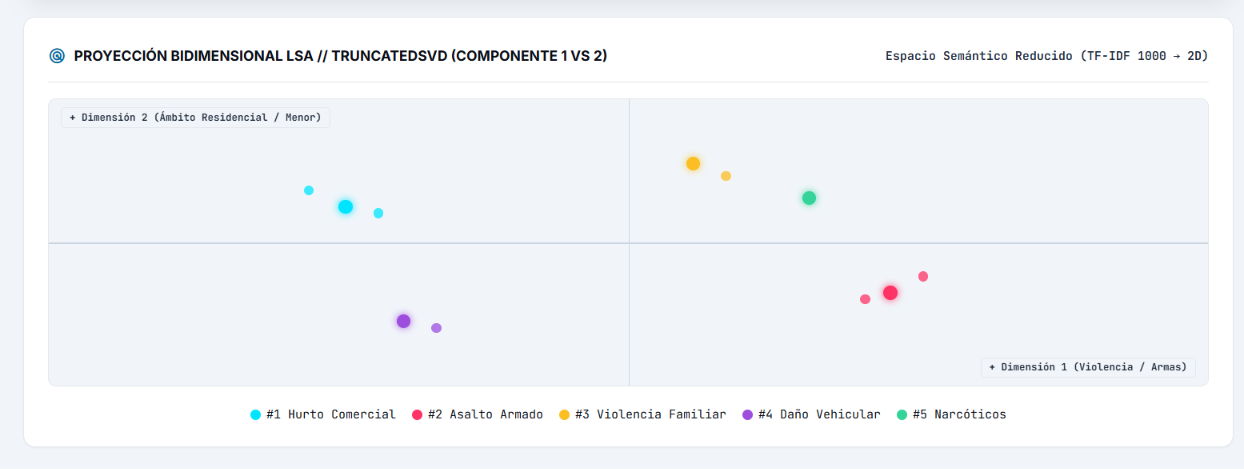
\includegraphics[width=0.88\textwidth]{figuras/imgProyeccionBidimensionalBolivia.png}
\caption{Proyección Bidimensional del Espacio Semántico Reducido LSA Mediante TruncatedSVD.}
\label{fig:lsa_proyeccion}
\figurenote{Captura del laboratorio analítico interactivo del proyecto. Ilustra la descomposición semántica latente ($1000 \to 2\text{D}$) sobre las crónicas de Bolivia, proyectando la Dimensión 1 (delitos armados y violencia callejera) frente a la Dimensión 2 (ámbito residencial y hurtos menores).}
\end{figure}

\subsubsection{Autoencoders Neuronales para Detección de Anomalías}

Un Autoencoder es una red neuronal artificial entrenada de modo no supervisado para reconstruir su propia entrada $x \in \mathbb{R}^D$ a través de un espacio latente comprimido $h \in \mathbb{R}^d$ ($d \ll D$):
\begin{equation}
    h = f(W_e x + b_e), \quad \hat{x} = g(W_d h + b_d)
\end{equation}
Al entrenarse sobre patrones comunes de criminalidad, la red minimiza la función de pérdida del error cuadrático medio (MSE):
\begin{equation}
    \mathcal{L}(x, \hat{x}) = \frac{1}{D} \sum_{j=1}^D (x_j - \hat{x}_j)^2
\end{equation}
Dado que las anomalías no siguen la distribución preponderante aprendida por los pesos neuronales, su reconstrucción sufre un error elevado. Se define el umbral de anomalía $\tau$ a partir del percentil 90 o de la cota estadística $\tau = \mu_{\text{MSE}} + 2.5 \sigma_{\text{MSE}}$, marcando como incidentes sospechosos o atípicos aquellos que cumplen $\mathcal{L}(x, \hat{x}) > \tau$.

\subsubsection{Modelado de Tópicos con Latent Dirichlet Allocation (LDA)}

LDA \cite{blei2003} es un modelo generativo probabilístico bayesiano que asume que cada documento (crónica periodística o reporte criminal) es una mezcla de tópicos latentes, y que cada tópico es una distribución sobre palabras del vocabulario. Dado el parámetro hiper-a priori de Dirichlet $\alpha$ para las mezclas de tópicos y $\beta$ para las distribuciones de palabras, la probabilidad conjunta de un documento es:
\begin{equation}
    p(\theta, z, w \mid \alpha, \beta) = p(\theta \mid \alpha) \prod_{n=1}^N p(z_n \mid \theta) \, p(w_n \mid z_n, \beta)
\end{equation}
Permite descubrir automáticamente temáticas emergentes como homicidios con armas de fuego, hurtos callejeros, microtráfico de drogas o delitos patrimoniales.

